\chapter{$G-$conjuntos y $p$-grupos}
\begin{definicion}
    Sea $G$ un grupo y $X$ un conjunto no vacío, una acción\footnote{En realidad esta es la definición de acción por la izquierda, pero no vamos a trabajar con las acciones por la derecha, por lo que hablaremos simplemente de acciones.} de $G$ sobre $X$ es una aplicación: 
    \Func{ac}{G\times X}{X}{(g,x)}{ac(g,x)}
    Que verifica:
    \begin{enumerate}
        \item[$i)$] $ac(1,x) = x$ $\quad \forall x\in X$.
        \item[$ii)$] $ac(g, ac(h, x)) = ac(gh, x)$ $\quad \forall x\in X, \quad \forall g,h\in G$.
    \end{enumerate}
    En dicho caso, diremos que $G$ actúa\footnote{En realidad deberíamos decir que ``$G$ actúa por la izquierda sobre $X$''.} (o que opera) sobre $X$.\\

    \noindent
    Si $G$ actúa sobre $X$, diremos que este conjunto $X$ es un $G-$conjunto a izquierda. A la aplicación $ac$ se le llama aplicación de la $G-$estructura.
\end{definicion}

\begin{notacion}
    Si $ac:G\times X\to X$ es una acción de $G$ sobre $X$, es común denotar:
    \begin{equation*}
        ac(g,x) = \prescript{g}{}{x} = g\cdot x = g\ast x
    \end{equation*}
    En este documento, usaremos la notación $ac(g,x) = \prescript{g}{}{x}$. Con esta, las propiedades que ha de cumplir una aplicación $ac:G\times X\to X$ para ser una acción son:
    \begin{enumerate}
        \item[$i)$] $\prescript{1}{}{x} = x$ $\forall x\in X$.
        \item[$ii)$] $\prescript{g}{}{(\prescript{h}{}{x})} = \prescript{gh}{}{x}$ $\forall x\in X$, $\forall g\in G$.
    \end{enumerate}
\end{notacion}

\begin{ejemplo}
    Si $G$ es un grupo y $X$ es un conjunto no vacío, ejemplos de acciones de $G$ sobre $X$ son:
    \begin{enumerate}
        \item La \underline{acción trivial}:
            \Func{ac}{G\times X}{X}{(g,x)}{x}
        \item Si tenemos una acción $ac:G\times X\to X$ y $H<G$, podemos considerar la \underline{acción por restricción} $ac:H\times X\to X$, dada por:
            \begin{equation*}
                ac(h,x) = ac(i(h),x) \qquad \forall h\in H, x\in X
            \end{equation*}
            Donde consideramos la aplicación inclusión $i:H\to G$ dada por $i(h) = h$, para todo $h\in H$.
        \item Dado $n\in \mathbb{N}$, si $X = \{1,\ldots,n\}$ y $G = S_n$, la \underline{acción natural} de $S_n$ sobre $X$ será la acción $ac:S_n\times X\to X$ dada por:
            \begin{equation*}
                ac(\sigma,k) = \prescript{\sigma}{}{k} = \sigma(k) \qquad \forall \sigma\in S_n, k\in X
            \end{equation*}
    \end{enumerate}
\end{ejemplo}

\begin{prop}\label{prop:accion_homomorfismo}
    Sea $G$ un grupo y $X$ un conjunto no vacío, dar una acción de $G$ sobre $X$ equivale a dar un homomorfismo de grupos de $G$ en $\Perm(X)$.
    \begin{proof}
        Veamos que es posible:
        \begin{itemize}
            \item Por una parte, dada una acción de $G$ sobre $X$, $ac:G\times X \to X$, podemos definir la aplicación: 
                \Func{\phi}{G}{\Perm(X)}{g}{\phi(g)}
                Donde $\phi(g)$ es una aplicación $\phi(g):X\longrightarrow X$ dada por:
                \begin{equation*}
                    \phi(g)(x) = \prescript{g}{}{x} \qquad \forall x\in X
                \end{equation*}
                Veamos en primer lugar que $\phi$ está bien definida, es decir, que $\phi(g) \in \Perm(X)$ para cada $g\in G$. Para ello, veamos antes que $\phi$ cumple:
                \begin{itemize}
                    \item $\phi(1) = id_X$, ya que la aplicación $x\mapsto ac(1,x)$ es la aplicación identidad en $X$, por ser $ac$ una acción de $G$ sobre $X$.
                    \item $\phi(g)\phi(h) = \phi(gh)$, ya que al evaluar en cualquier $x\in G$:
                        \begin{equation*}
                            (\phi(g)\phi(h))(x) = \phi(g)(\phi(h)(x)) = \phi(g)(\prescript{h}{}{x}) = \prescript{g}{}{(\prescript{h}{}{x})} \AstIg \prescript{gh}{}{x} = \phi(gh)(x)
                        \end{equation*}
                        Donde en $(\ast)$ hemos usado que $ac$ es una acción de $G$ sobre $X$.
                \end{itemize}
                Ahora, veamos que dado $g\in G$, la aplicación $\phi(g)$ es biyectiva (es decir, está en $\Perm(X)$), ya que su aplicación inversa es $\phi(g^{-1})$:
                \begin{equation*}
                    \phi(g^{-1})\phi(g) = \phi(g^{-1}g) = \phi(1) = \phi(gg^{-1}) = \phi(g) \phi(g^{-1})
                \end{equation*}
                Y anteriormente vimos que $\phi(1) = id_X$, por lo que $\phi(g) \in \Perm(X)$, para todo $g\in G$ y la aplicación $\phi$ está bien definida.\\

                \noindent
                Además, por las dos propiedades anteriores, tenemos que $\phi$ es un homomorfismo de grupos.
            \item Sea $\phi:G\to \Perm(X)$ un homomorfismo de grupos, definimos la aplicación $ac:G\times X \to X$ dada por:
                \begin{equation*}
                    ac(g,x) = \phi(g)(x) \qquad \forall g\in G, x\in X
                \end{equation*}
                Veamos que es una acción:
                \begin{align*}
                    ac(1,x) &= \phi(1)(x) = id_X(x) = x \qquad \forall x\in X \\
                    ac(g,ac(h,x)) &= \phi(g)(\phi(h)(x)) = (\phi(g)\phi(h))(x) = \phi(gh)(x) = ac(gh,x)  \\ &\forall x\in X, \quad \forall g,h\in G
                \end{align*} \qedhere
        \end{itemize}
    \end{proof}
\end{prop}

\begin{definicion}[Representación por permutaciones]
    Sea $G$ un grupo y $X$ un conjunto no vacío, si tenemos una acción de $G$ sobre $X$, el homomorfismo $\phi$ dado por esta acción según la Proposición~\ref{prop:accion_homomorfismo} recibirá el nombre de \underline{representación de $G$ por} \underline{permutaciones}.\\

    \noindent
    Además, llamaremos a $\ker(\phi)$ \underline{núcleo de la acción}, ya que:
    \begin{equation*}
        \ker(\phi) = \{g\in G \mid \phi(g) = id_X\} = \{g\in G \mid \prescript{g}{}{x} = x \quad \forall x\in X\}
    \end{equation*}
    En el caso de que $\ker(\phi) = \{1\}$, diremos que la acción es \underline{fiel}.
\end{definicion}

\begin{ejemplo}
    A continuación, dados varios ejemplos de acciones, consideraremos en cada caso su representación por permutaciones:
    \begin{enumerate}
        \item La representación por permutaciones de la acción trivial es el homomorfismo $\phi:G\to Perm(X)$ dado por:
            \begin{equation*}
                \phi(g) = id_X \qquad \forall g\in G
            \end{equation*}
        \item Si tenemos un conjunto no vacío $X$ y una acción $ac:G\times X\to X$ sobre un grupo $G$ que tiene asociada una representación por permutaciones $\phi$, entonces la acción por restricción $ac:H\times X\to X$ tendrá asociada como representación por permutaciones el homomorfismo $\phi_H:H\to Perm(X)$ dado por:
            \begin{equation*}
                \phi_H = \phi \circ i 
            \end{equation*}
            Siendo $i:H\to G$ la aplicación inclusión.
        \item En el caso de la acción natural de $S_n$ sobre $X =\{1,\ldots,n\} $, tenemos que la representación por permutaciones es el homomorfismo $\phi:S_n\to S_n$ dado por:
            \begin{equation*}
                \phi(\sigma) = \sigma \qquad \forall \sigma\in S_n
            \end{equation*}
            Es decir, $\phi = id_{S_n}$.
        \item Sea $G$ un grupo, podemos definir la \underline{acción por traslación} como:
            \Func{ac}{G\times G}{G}{(g,h)}{gh}
            Y el homomorfismo asociado a la acción como representación por permutaciones será $\phi:G\to \Perm(G)$ dado por:
            \begin{equation*}
                \phi(g)(h) = gh \qquad \forall g,h\in G
            \end{equation*}
            Como además:
            \begin{equation*}
                \ker(\phi) = \{g\in G\mid gh = h \quad \forall h\in G\} = \{1\}
            \end{equation*}
            Tenemos que es una acción fiel.
    \end{enumerate}
\end{ejemplo}

\begin{teo}[Cayley] % // TODO: Poner tmb para grupos no finitos
    Todo grupo es isomorfo a un subgrupo de un grupo de permutaciones.
    \begin{proof}
        Sea $G$ un grupo, consideramos la acción por traslación:
        \Func{ac}{G\times G}{G}{(g,h)}{gh}
        Y su representación por permutaciones, $\phi:G\to \Perm(G)$ dado por:
        \begin{equation*}
            \phi(g)(h) = gh \qquad \forall g\in G, \forall h\in G
        \end{equation*}
        Como la acción por traslación es una acción fiel, tendremos que $\ker(\phi) = \{1\}$ y aplicando el Primer Teorema de Isomorfía sobre $\phi$, obtenemos que:
        \begin{equation*}
            G \cong G/\{1\} \cong Im(\phi)
        \end{equation*}
        Donde $Im(\phi) = \phi_\ast(G)$, que en la Proposición~\ref{prop:imagen_directa} vimos que es un subgrupo de $\Perm(G)$.
    \end{proof}
\end{teo}

\begin{ejemplo}
    Podemos considerar las traslaciones de $G$ sobre conjuntos especiales:
    \begin{itemize}
        \item La acción por traslación de $G$ sobre $\cc{P}(G)$ será $ac:G\times \cc{P}(G) \to \cc{P}(G)$ dada por:
            \begin{equation*}
                ac(g,A) = gA = \{ga \mid a\in A\}  \subseteq G \qquad \forall A\in \cc{P}(G)
            \end{equation*}
        \item Podemos también considerar la acción por traslación en el cociente por las clases laterales por la izquierda\footnote{No es necesario considerar $H\lhd G$, ya que solo consideramos conjuntos no vacíos, por lo que no es necesario que el cociente tenga estructura de grupo.}: si $H<G$, consideramos el cociente de $G$ sobre $H$ por la izquierda y la acción $ac:G\times G/\prescript{}{H}{\sim} \to G/\prescript{}{H}{\sim}$ dada por:
            \begin{equation*}
                ac(g,xH) = \prescript{g}{}{(xH)} = gxH  = \{gxh \mid h\in H\}
            \end{equation*}
    \end{itemize}
    \begin{enumerate}
        \item[6.] La \underline{acción por conjugación} se define como $ac:G\times G\to G$ dada por:
            \begin{equation*}
                ac(g,h) = \prescript{g}{}{h} = ghg^{-1}
            \end{equation*}
            Que es una acción, ya que:
            \begin{align*}
                \prescript{1}{}{h} &= 1h1^{-1} = h \qquad \forall h\in G\\
                \prescript{g}{}{(\prescript{h}{}{l})} &= g\prescript{h}{}{l}g^{-1} = ghlh^{-1}g^{-1} = ghl{(gh)}^{-1} = \prescript{gh}{}{l} \qquad \forall g,h,l \in G
            \end{align*}
            El homomorfismo asociado es:
            \begin{gather*}
                \phi:G\to\Perm(G) \\
                \phi(g)(h) = ghg^{-1} \qquad \forall g,h\in G
            \end{gather*}
            El núcleo en este caso es:
            \begin{equation*}
                \ker(\phi) = \{g\in G \mid ghg^{-1} = h \quad \forall h\in G\} = \{g\in G \mid gh = hg \quad \forall h\in G\} = Z(G)
            \end{equation*}
        \item[7.] La \underline{acción por conjugación en partes de $G$} se define como la aplicación \newline $ac:G\times \cc{P}(G) \to \cc{P}(G)$ dada por:
            \begin{equation*}
                ac(g,A) = \prescript{g}{}{A} = gAg^{-1} = \{gag^{-1} \mid a\in A\} \subseteq G \qquad \forall A\in \cc{P}(G)
            \end{equation*}
        \item[8.] Podemos definir la acción por conjugación de $G$ también sobre $Subg(G)$:
            \begin{equation*}
                Subg(G) = \{H\subseteq G \mid H<G\}
            \end{equation*}
            Como la aplicación $ac:G\times Subg(G) \to Subg(G)$ dada por:
            \begin{equation*}
                ac(g,H) = \prescript{g}{}{H} = gHg^{-1} < G
            \end{equation*}
            Ya que en la Proposición~\ref{prop:xHx_subgrupo} vimos que $gHg^{-1}$ era un subgrupo de $G$, al que llamaremos subgrupo conjugado de $G$.
    \end{enumerate}
\end{ejemplo}

\section{Órbitas de un elemento}

\begin{definicion}[Órbita]
    Sea $G$ un grupo y $X$ un $G-$conjunto, definimos en $X$ una relación de equivalencia $\sim$ (se comprueba a continuación) dada por:
    \begin{equation*}
        y\sim x \Longleftrightarrow \exists g\in G \mid y = \prescript{g}{}{x}
    \end{equation*}
    La clase de equivalencia de cada $x\in X$ se llama \underline{órbita de $x$}, denotada por:
    \begin{equation*}
        Orb(x) = \{y\in X \mid \exists g\in G \text{\ con\ } y=\prescript{g}{}{x}\}
    \end{equation*}
    Como estamos considerando una acción, será equivalente escribir (gracias a la propiedad simétrica):
    \begin{equation*}
        Orb(x) = \{y\in X\mid \exists g\in G \text{\ con\ } \prescript{g}{}{y} = x\}
    \end{equation*}
    Tenemos de esta forma que el conjunto cociente $X/\sim$ es el conjunto formado por las órbitas de todos los elementos de $X$:
    \begin{equation*}
        X/\sim\ = \{Orb(x) \mid x\in X\}
    \end{equation*}
\end{definicion}
\begin{prop}
    La relación $\sim$ de la definición anterior es una relación de equivalencia en $X$.
    \begin{proof}
        Comprobamos la reflexividad, simetría y transitividad de $\sim$:
        \begin{itemize}
            \item[$i)$] \ul{Reflexividad}: sea $x\in X$, entonces $\prescript{1}{}{x} = x$, por lo que $x\sim x$.
            \item[$ii)$] \ul{Simetría}: sean $x,y\in X$ tales que $y\sim x$, entonces $\exists g\in G$ de forma que $y = \prescript{g}{}{x}$. Como $G$ es un grupo, consideramos $g^{-1}\in G$, de forma que:
                \begin{equation*}
                    \prescript{g^{-1}}{}{y} = \prescript{g^{-1}}{}{(\prescript{g}{}{x})} = \prescript{g^{-1}g}{}{x} = \prescript{1}{}{x} = x
                \end{equation*}
            Por lo que $x\sim y$.
            \item[$iii)$] \ul{Transitividad}: sean $x,y,z\in X$ tales que $x\sim y$ e $y\sim z$, entonces $\exists g,h\in G$ de forma que:
                \begin{align*}
                    y = \prescript{g}{}{x} \hspace{2cm}
                    z = \prescript{h}{}{y}
                \end{align*}
                Entonces, tenemos que:
                \begin{equation*}
                    z = \prescript{h}{}{(\prescript{g}{}{x})} = \prescript{hg}{}{x}
                \end{equation*}
                Como $hg\in G$, tenemos que $z\sim x$.\qedhere
        \end{itemize}
    \end{proof}
\end{prop}

\begin{ejemplo}
    Sobre $X = \{1,2,3,4\}$:
    En $S_4$ consideramos $ac:S_4\times X\to X$, la acción natural de $S_4$ sobre $X$:
        \begin{equation*}
            ac(\sigma,k) = \prescript{\sigma}{}{k} = \sigma(k)
        \end{equation*}
    \begin{itemize}
        \item Si tenemos $H = \langle (1\ 2\ 3) \rangle $, queremos calcular las órbitas de los elementos de $X$. Recordamos que:
            \begin{equation*}
                Orb(x) = \{y\in X \mid \exists \sigma\in H \text{\ con\ } \sigma(y) = x\}
            \end{equation*}
            Es decir, pensamos en $Orb(x)$ como en los elementos de $X$ desde los que podemos llegar a $x$ con una permutación de $H$ (o también como en aquellos elementos de $X$ desde los que podemos llegar a $x$ a través de una permutación de $H$). De esta forma:
            \begin{align*}
                Orb(1) &= \{1,2,3\} \\
                Orb(2) &= \{1, 2, 3\} \\
                Orb(3) &= \{1, 2, 3\} \\
                Orb(4) &= \{4\}
            \end{align*}
        \item En $A_4$:
            \begin{multline*}
                A_4 = \{1, (1\ 2)(3\ 4), (1\ 3)(2\ 4), (1\ 4)(2\ 3), (1\ 2\ 3), (1\ 2\ 4), (1\ 3\ 4), (2\ 3\ 4), (1\ 3\ 2),\\ (1\ 4\ 2), (1\ 4\ 3), (2\ 4\ 3)\}
            \end{multline*}
            Como tenemos todos los $3-$ciclos:
            \begin{equation*}
                Orb(1) = X
            \end{equation*}
            Y también tendremos que $Orb(k) = X$, para $k\in X$.
        \item En $V$, que contiene a todos los $2-$ciclos, la situación será la misma:
            \begin{equation*}
                Orb(k) = X \qquad \forall k\in X
            \end{equation*}
        \item En $H = \langle (1\ 2\ 3\ 4) \rangle $ sucede lo mismo:
            \begin{equation*}
                Orb(k) = X \qquad \forall k\in X
            \end{equation*}
    \end{itemize}
\end{ejemplo}

\begin{definicion}
    Si el conjunto de órbitas $X/\sim$ es unitario, decimos que la acción es \underline{transitiva}.\\

    \noindent
    Este nombre se debe a que dados $x,y\in X$, siempre $\exists g\in G$ de forma que:
    \begin{equation*}
        y = \prescript{g}{}{x}
    \end{equation*}
\end{definicion}

\begin{definicion}[Estabilizador]
    Sea $G$ un grupo y $X$ un $G-$conjunto, definimos el grupo de estabilizadores de $x\in X$ en $G$ como:
    \begin{equation*}
        Stab_G(x) = \{g\in G \mid \prescript{g}{}{x} = x\}
    \end{equation*}
    También se le llama grupo de isotropía.
\end{definicion}

\noindent
Para justificar por qué a $Stab_G(x)$ le llamábamos \underline{grupo} de estabilizadores de $x$ en $G$, es necesaria la siguiente Proposición:
\begin{prop}
    Sea $G$ un grupo y $X$ un $G-$conjunto:
    \begin{equation*}
        Stab_G(x) < G \qquad \forall x\in X
    \end{equation*}
    \begin{proof}
        Fijado $x\in X$, es claro que $Stab_G(x) \subseteq G$. Vemos que:
        \begin{itemize}
            \item $1\in Stab_G(x)$, ya que $\prescript{1}{}{x} = x$ por definición de acción.
            \item Si $g\in Stab_G(x)$, supongamos que $g^{-1}\notin Stab_G(x)$, con lo que $\prescript{g^{-1}}{}{x} = y \in X$ con $y\neq x$. En dicho caso:
                \begin{equation*}
                    x = \prescript{1}{}{x} = \prescript{g^{-1}g}{}{x} = \prescript{g^{-1}}{}{(\prescript{g}{}{x})} = \prescript{g^{-1}}{}{x} = y
                \end{equation*}
                Llegamos a una \underline{contradicción}, luego $g^{-1}\in Stab_G(x)$ para todo $g\in Stab_G(x)$.
            \item Finalmente, si $g,h\in Stab_G(x)$, entonces:
                \begin{equation*}
                    \prescript{gh}{}{x} = \prescript{g}{}{(\prescript{h}{}{x})} = \prescript{g}{}{x} = x
                \end{equation*}
                Por lo que $gh \in Stab_G(x)$.
        \end{itemize}
    \end{proof}
\end{prop}

\begin{ejemplo}
    Si nuevamente sobre $X = \{1,2,3,4\}$ volvemos a considerar la acción natural de $S_4$ sobre $X$:
    \begin{itemize}
        \item En $H = \langle (1\ 2\ 3) \rangle $, recordamos que:
            \begin{equation*}
                Stab_H(x) = \{\sigma\in H \mid \sigma(x) = x\}
            \end{equation*}
            Es decir, el grupo de estabilizadores de $x$ en $H$ son los elementos de $H$ que dejan fijo el elemento $x$. De esta forma:
            \begin{align*}
                Stab_H(1) &= \{1\} \\
                Stab_H(2) &= \{1\} \\
                Stab_H(3) &= \{1\} \\
                Stab_H(4) &= H
            \end{align*}
        \item En $A_4$:
            \begin{align*}
                Stab_{A_4}(1) &= \{1, (2\ 3\ 4), (2\ 4\ 3)\} = \langle (2\ 3\ 4) \rangle  \\
                Stab_{A_4}(2) &= \langle (1\ 3\ 4) \rangle  \\
                Stab_{A_4}(3) &= \langle (1\ 2\ 4) \rangle  \\
                Stab_{A_4}(4) &= \langle (1\ 2\ 3) \rangle  
            \end{align*}
        \item En $V$:
            \begin{equation*}
                Stab_V(k) = \{1\} \qquad \forall k\in X
            \end{equation*}
        \item En $H = \langle (1\ 2\ 3\ 4) \rangle $:
            \begin{equation*}
                Stab_H(k) = \{1\} \qquad \forall k\in X
            \end{equation*}
    \end{itemize}
\end{ejemplo}

% // TODO: Ver si dejo esto
\noindent
Vamos a poder establecer una relación entre el órden de las órbitas y del conjunto cociente.

\begin{prop}\label{prop:orb_stab}
   Sea $G$ un grupo finito que actúa sobre $X$, entonces para cada $x\in X$, $Orb(x)$ es un conjunto finito y:
   \begin{equation*}
       |Orb(x)| = [G:Stab_G(x)]
   \end{equation*}
   En particular, el cardinal de la órbita es un divisor del orden de $G$.
   \begin{proof}
       Fijado $x\in X$, si consideramos $Stab_G(x) < G$ y las clases laterales por la izquierda\footnote{No consideramos el conjunto cociente porque no sabemos si $Stab_G(x)$ es un subgrupo normal en $G$ o no.}, $G/\prescript{}{Stab_G(x)}{\sim}$, definimos la aplicación $\phi:G/\prescript{}{Stab_G(x)}{\sim}\longrightarrow Orb(x)$ dada por:
       \begin{equation*}
           \phi(gStab_G(x)) = \prescript{g}{}{x} \qquad \forall gStab_G(x) \in G/\prescript{}{Stab_G(x)}{\sim}
       \end{equation*}
       \begin{itemize}
           \item Veamos que está bien definida. Para ello, sean $g,g' \in G$ de forma que:
               \begin{equation*}
                   gStab_G(x) = g'Stab_G(x)
               \end{equation*}
               Entonces, existirá $h\in Stab_G(x)$ de forma que $g = g'h$. En dicho caso:
               \begin{equation*}
                   \phi(gStab_G(x)) = \prescript{g}{}{x} = \prescript{g'h}{}{x} = \prescript{g'}{}{(\prescript{h}{}{x})} = \prescript{g'}{}{x} = \phi(g'Stab_G(x))
               \end{equation*}
           \item Veamos que es sobreyectiva: sea $y\in Orb(x)$, entonces $\exists g\in G$ de forma que:
               \begin{equation*}
                   y = \prescript{g}{}{x}
               \end{equation*}
               Por lo que $y = \phi(gStab_G(x))$.
           \item Para la inyectividad, sean $g,g'\in G$ de forma que:
               \begin{equation*}
                   \prescript{g}{}{x} = \phi(gStab_G(x)) = \phi(g'Stab_G(x)) = \prescript{g'}{}{x}
               \end{equation*}
               Entonces, podemos escribir:
               \begin{equation*}
                   x = \prescript{g^{-1}}{}{(\prescript{g}{}{x})} = \prescript{g^{-1}}{}{(\prescript{g'}{}{x})} = \prescript{g^{-1}g'}{}{x}
               \end{equation*}
               De donde concluimos que $g^{-1}g'\in Stab_G(x)$, por lo que $gStab_G(x) = g'Stab_G(x)$.
       \end{itemize}
       En definitiva, acabamos de probar que $Orb(x)$ es biyectivo con $G/\prescript{}{Stab_G(x)}{\sim}$, por lo que tienen el mismo cardinal. Además:
       \begin{itemize}
           \item Por ser $G$ finito y $Stab_G(x)<G$, tenemos que:
               \begin{equation*}
                   |Orb(x)| = [G:Stab_G(x)] = \dfrac{|G|}{|Stab_G(x)|}
               \end{equation*}
               Por lo que $Orb(x)$ es un conjunto finito.
           \item Despejando de la igualdad superior, tenemos que:
               \begin{equation*}
                   |Orb(x)||Stab_G(x)| = |G|
               \end{equation*}
               Por lo que $|Orb(x)|$ es un divisor de $|G|$.
       \end{itemize}
   \end{proof}
\end{prop}

\begin{observacion}
La demostración es cierta sin suponer que $G$ sea un grupo finito, pero entonces solo podemos poner como tesis que $Orb(x)$ es biyectivo con $G/\prescript{}{Stab_G(x)}{\sim}$, para todo $x\in X$.
\end{observacion}

\begin{prop}
    Sea $G$ un grupo que actúa sobre $X$, si $x,y\in X$ están en la misma órbita, entonces $Stab_G(x)$ y $Stab_G(y)$ son subgrupos conjugados.
    \begin{proof}
        Si $x$ e $y$ están en la misma órbita, entonces $Orb(x) = Orb(y)$, por lo que $\exists g\in G$ de forma que $y = \prescript{g}{}{x}$. En dicho caso, también tenemos que $x = \prescript{g^{-1}}{}{y}$. Veamos que:
        \begin{equation*}
            Stab_G(x) = g^{-1}Stab_G(y)g
        \end{equation*}
        Para ello:
        \begin{description}
            \item[$\subseteq)$] Sea $h\in Stab_G(x)$, queremos ver que $h\in g^{-1}Stab_G(y)g$, para lo que bastará ver que $ghg^{-1}\in Stab_G(y)$:
                \begin{equation*}
                    \prescript{ghg^{-1}}{}{y} = \prescript{gh}{}{x} = \prescript{g}{}{x} = y
                \end{equation*}
            \item[$\supseteq)$] Sea $h\in Stab_G(y)$, queremos ver que $g^{-1}hg\in Stab_G(x)$:
                \begin{equation*}
                    \prescript{g^{-1}hg}{}{x} = \prescript{g^{-1}h}{}{y} = \prescript{g^{-1}}{}{y} = x
                \end{equation*}
        \end{description}
    \end{proof}
\end{prop}

\begin{definicion}
    Sea $G$ un grupo y $X$ un $G-$conjunto, un elemento $x\in X$ se dice que es \underline{fijo} por la acción si $\prescript{g}{}{x} = x$, $\forall g\in G$.\\

    \noindent
    Consideramos el conjunto de todos los elementos que se quedan fijos por todos los elementos de $G$:
    \begin{equation*}
        Fix(X) = \{x\in X \mid \prescript{g}{}{x} = x, \quad \forall g\in G\}
    \end{equation*}
\end{definicion}

\begin{prop}
    Sea $G$ un grupo y $X$ un $G-$conjunto, si $x\in X$, entonces:
    \begin{equation*}
        x\in Fix(X) \Longleftrightarrow Orb(x) = \{x\} \Longleftrightarrow Stab_G(x) = G
    \end{equation*}
    \begin{proof}
        Si recordamos las definiciones de estos tres conjuntos:
        \begin{align*}
            Orb(x) &= \{y\in X \mid \exists g\in G \text{\ con\ } \prescript{g}{}{y} = x\} \\
            Stab_G(x) &= \{g\in G \mid \prescript{g}{}{x} = x\} \\
            Fix(X) &= \{x\in X \mid \prescript{g}{}{x} = x \quad \forall g\in G\}
        \end{align*}
        Veamos todas las implicaciones:
        \begin{description}
            \item [$x\in Fix(X) \Longrightarrow Orb(x) = \{x\}$]~\\
                Si $y\in Orb(x)$, entonces $\exists g\in G$ con $\prescript{g}{}{y}= x$, por lo que:
                \begin{equation*}
                    y = \prescript{g^{-1}g}{}{y} = \prescript{g^{-1}}{}{(\prescript{g}{}{y})} = \prescript{g^{-1}}{}{x} \AstIg x
                \end{equation*}
                Donde en $(\ast)$ usamos que $x\in Fix(X)$. Concluimos que $Orb(x) = \{x\}$.
            \item [$Orb(x) = \{x\} \Longrightarrow Stab_G(x) = G$]~\\
                Sea $g\in G$, si consideramos  $y = \prescript{g}{}{x}$, entonces $y\in Orb(x) = \{x\}$, de donde $y = x$ y $g\in Stab_G(x)$.
            \item [$Stab_G(x) = G \Longrightarrow x\in Fix(x)$]~\\
                \begin{equation*}
                    \prescript{g}{}{x} = x \qquad \forall g\in G
                \end{equation*}
                De donde deducimos que $x\in Fix(X)$.
        \end{description}
    \end{proof}
\end{prop}

\begin{observacion}
    Si tenemos un grupo $G$ y un $G-$conjunto $X$, recordamos que tenemos definida sobre $X$ una relación de equivalencia $\sim$, con la que anteriormente definimos los órbitas de los elementos. En el caso de que $X$ sea un conjunto finito y tenga $n$ elementos:
    \begin{equation*}
        X = \{x_1, \ldots, x_n\}
    \end{equation*}
    Por ser $\sim$ una relación de equivalencia, tenemos una partición de $X$, lo que nos da la igualdad:
    \begin{equation*}
        |X| = \sum_{k=1}^{n}|Orb(x_k)|
    \end{equation*}
    Para simplificarla usando propiedades ya vistas, sabemos que puede haber órbitas unitarias:
    \begin{equation*}
        Orb(x) = \{x\} \Longleftrightarrow x\in Fix(x)
    \end{equation*}
    Por tanto, podemos simplificar la igualdad superior, eliminando de ella todas las órbitas unitarias. Para ello, si $\Gamma$ contiene un único representante de cada una de las órbitas de elementos que no son puntos fijos ($\Gamma\subseteq X\setminus Fix(X)$):
    \begin{equation*}
        |X| = \sum_{k=1}^{n}|Orb(x_k)| = |Fix(X)| + \sum_{y\in \Gamma}|Orb(y)|
    \end{equation*}
    Y aplicando finalmente la Proposición~\ref{prop:orb_stab}, llegamos a que:
    \begin{equation*}
        |X| = \sum_{k=1}^{n}|Orb(x_k)| = |Fix(X)| + \sum_{y\in \Gamma}|Orb(y)| = |Fix(X)| + \sum_{y\in \Gamma} [G:Stab_G(y)]
    \end{equation*}
\end{observacion}

\noindent
A continuación, lo que haremos será estudiar los conjuntos $Orb(\cdot )$, $Stab_G(\cdot )$ y $Fix(X)$ para ciertos ejemplos comunes de acciones.
\subsection{Acción por traslación}
\noindent
Sea $G$ un grupo no trivial, la acción por traslación se define como $ac:G\times G\to G$ dada por:
\begin{equation*}
    ac(g,h) = \prescript{g}{}{h} = gh \qquad \forall g,h\in G
\end{equation*}
De esta forma, tenemos que:
\begin{equation*}
    Orb(h) = \{k\in G \mid \exists g\in G \text{\ con\ } k = \prescript{g}{}{h} = gh\} = G \qquad \forall h\in G
\end{equation*}
Ya que fijado $k\in G$ y dado $h\in G$, siempre podemos tomar $g = kh^{-1}\in G$ para tener que $\prescript{g}{}{h} = gh = k$.
\begin{align*}
    Stab_G(h) &= \{g\in G \mid gh = \prescript{g}{}{h} = h\} = \{1\} \qquad \forall h\in G\\
    Fix(G) &= \{h\in G \mid gh = \prescript{g}{}{h}=h \quad \forall g\in G\} = \emptyset 
\end{align*}

\begin{observacion}
    Observemos que la acción por traslación cuenta con las mismas cualidades que tiene una traslación entre dos espacios vectoriales, pensando en que primero fijamos un vector $v\in V$ para luego definir una aplicación $t_v:V\to V'$. De esta forma:
    \begin{itemize}
        \item Fijado cualquier vector $v$, $t_v$ siempre será sobreyectiva. Esto se pone de manifiesto al decir que $Orb(h) = G$ para todo $h\in G$.
        \item La única traslación que mantiene fijo un punto es la correspondiente al vector 0, que deja fijos todos los puntos, $Stab_G(h) = \{1\}$ $\forall h\in G$.
        \item Como hay traslaciones que no mantienen fijos ningún punto (todas salvo la trivial), no hay ningún punto que permanezca invariante ante todas ellas, $Fix(G) = \emptyset $.
    \end{itemize}
\end{observacion}

\subsection{Acción por conjugación}
\noindent
Sea $G$ un grupo, la acción por conjugación se define como $ac:G\times G\to G$ dada por:
\begin{equation*}
    ac(g,h) = \prescript{g}{}{h} = ghg^{-1} \qquad \forall g,h\in G
\end{equation*}

\subsubsection{Preliminares}
\noindent
Antes de estudiar los subconjuntos notables de esta acción, definimos ciertos conjuntos y vemos propiedades de estos que nos ayudarán a entender la acción.

\begin{definicion}[Centralizador]
    Sea $G$ un grupo y $S\subseteq G$, llamamos centralizador de $S$ en $G$ al conjunto:
    \begin{equation*}
        C_G(S) = \{x\in G \mid xs = sx \quad \forall s\in S\}
    \end{equation*}
\end{definicion}

\begin{definicion}[Normalizador]
    Sea $G$ un grupo y $S\subseteq G$, llamamos normalizador de $S$ en $G$ al conjunto:
    \begin{equation*}
        N_G(S) = \{x\in G \mid xS = Sx\}
    \end{equation*}
\end{definicion}

\begin{prop}~\label{prop:normalizador} % // TODO: Ej 30 relacion 4
    Sea $G$ un grupo y $S\subseteq G$, se verifica:
    \begin{enumerate}
        \item[$i)$] $N_G(S) < G$.
        \item[$ii)$] $C_G(S) \lhd N_G(S)$.
        \item[$iii)$] Si $S<G$, entonces $S\lhd N_G(S)$.
    \end{enumerate}
    \begin{proof}
        Demostramos cada apartado:
        \begin{enumerate}
            \item[$i)$] Sean $x,y\in N_G(S)$, entonces tendremos que:
                \begin{align*}
                    xS &= Sx \Longrightarrow xSx^{-1} = S \\
                    yS &= Sy \Longrightarrow S = y^{-1}Sy
                \end{align*}
                En dicho caso:
                \begin{equation*}
                    (xy^{-1})S{(xy^{-1})}^{-1} = (xy^{-1})S(yx^{-1}) = x(y^{-1}Sy)x^{-1} = xSx^{-1} = S
                \end{equation*}
                De donde deducimos que $(xy^{-1})S = S(xy^{-1})$, por lo que $xy^{-1}\in N_G(S)$ y $N_G(S) < G$.
            \item[$ii)$] Hemos de ver primero que $C_G(S) < N_G(S)$:
                \begin{itemize}
                    \item En primer lugar, si $x\in C_G(S)$:
                        \begin{equation*}
                            xS = \{xs \mid s\in S\} = \{sx \mid s\in S\} = Sx
                        \end{equation*}
                        Por lo que $x\in N_G(S)$ y se tiene que $C_G(S) \subseteq N_G(S)$.
                    \item Ahora, si $x,y\in C_G(S)$, entonces:
                        \begin{align*}
                            xs &= sx \Longrightarrow xsx^{-1} = s \\
                            ys &= sy \Longrightarrow s = y^{-1}sy \qquad \forall s\in S
                        \end{align*}
                        Lo que nos permite escribir:
                        \begin{equation*}
                            (xy^{-1})s{(xy^{-1})}^{-1} = x(y^{-1}sy)x^{-1} = xsx^{-1} = s \qquad \forall s\in S
                        \end{equation*}
                        De donde deducimos que $xy^{-1}\in C_G(S)$, por lo que $C_G(S) < N_G(S)$.
                \end{itemize}
                Para la normalidad, dado $x\in C_G(S)$ y $g\in N_G(S)$, queremos ver que se cumple $y = gxg^{-1}\in C_G(S)$. Para ello, dado $s\in S$, vemos que:
                \begin{equation*}
                    ys = (gxg^{-1})s \AstIg gxs'g^{-1} = gs'xg^{-1} \stackrel{(\ast\ast)}{=} s(gxg^{-1}) = sy
                \end{equation*}
                Donde en $(\ast)$ usamos que como $g\in N_G(S)$, también tenemos que $g^{-1}\in N_G(S)$, con lo que $\exists s' \in S$ de forma que:
                \begin{equation*}
                    g^{-1}s = s'g^{-1}
                \end{equation*}
                Y en $(\ast\ast)$ deshacemos este proceso, ya que multiplicando la igualdad superior por derecha e izquierda por $g$, llegamos a que:
                \begin{equation*}
                    g^{-1}s = s'g^{-1} \Longrightarrow gg^{-1}sg = gs'g^{-1}g \Longrightarrow sg = gs'
                \end{equation*}
                En definitiva, de $ys = sy$ deducimos que $y = gxg^{-1}\in C_G(S)$, para todo $x\in C_G(S)$ y todo $g\in N_G(S)$, de donde $C_G(S)\lhd N_G(S)$.
            \item[$iii)$] Si suponemos además que $S<G$, por una parte tenemos que:
                \begin{equation*}
                    sS = S = Ss \qquad \forall s\in S
                \end{equation*}
                De donde deducimos que $S\subseteq N_G(S)$ y por ser $S<G$, tenemos que $S < N_G(S)$. Para la normalidad, si $g\in N_G(S)$, tendremos entonces que:
                \begin{equation*}
                    gS = Sg \Longrightarrow gSg^{-1} = S
                \end{equation*}
                De donde deducimos que $S \lhd N_G(S)$.
        \end{enumerate}
    \end{proof}
\end{prop}

\begin{prop} % // TODO: Ej 31 relacion 4
    Sea $G$ un grupo, $H,K< G$ con $H\subseteq K$, entonces:
    \begin{equation*}
        H \lhd K \Longleftrightarrow K < N_G(H)
    \end{equation*}
    De esta forma, el normalizador $N_G(H)$ se caracteriza como el mayor subgrupo de $G$ en el que $H$ es normal.
    \begin{proof}
        Por ser $H,K<G$ con $H\subseteq K$, tenemos ya que $H<K$. Por una caracterización que vimos de los subgrupos normales:
        \begin{equation*}
            H\lhd K \Longleftrightarrow kHk^{-1} = H \quad \forall k\in K \Longleftrightarrow kH = Hk \quad \forall k\in K \Longleftrightarrow K \subseteq N_G(H) 
        \end{equation*}
        Y por ser $K<G$, $K\subseteq N_G(H) \Longleftrightarrow K<N_G(H)$.
    \end{proof}
\end{prop}

\begin{ejercicio*}
    Para terminar de comprender las propiedades del centralizador y del normalizador, se pide probar que si $G$ es un grupo y $H<G$:
    \begin{align*}
        H\lhd G &\Longleftrightarrow G = N_G(H) \\
        H\subseteq Z(G) &\Longleftrightarrow G = C_G(H)
    \end{align*}
\end{ejercicio*}

\subsubsection{Subconjuntos notables}
\noindent
Estudiadas ya las propiedades del centralizador y del normalizador, estamos ya en condiciones de estudiar los conjuntos notables de la acción por conjugación:
\begin{equation*}
    Orb(h) = \{k\in G \mid \exists g\in G \text{\ con\ } k = \prescript{g}{}{h} = ghg^{-1}\} = \{ghg^{-1}\mid g\in G\} = Cl_G(h) \qquad \forall h\in G
\end{equation*}
De esta forma, llamaremos a la órbita de $h$ por la acción por conjugación la \underline{clase de} \underline{conjugación de $h$ en $G$}.
\begin{equation*}
    Stab_G(h) = \{g\in G \mid \prescript{g}{}{h} = ghg^{-1} = h\} = \{g \in G \mid gh = hg\} = C_G(h)
\end{equation*}
El estabilizador de $h$ en $G$ coincide con el centralizador de $h$ en $G$, y como la órbita de $h$ coincidía con la clase de conjugación de $h$ en $G$, por la Proposición~\ref{prop:orb_stab}, tenemos que:
\begin{equation*}
    |Cl_G(h)| = |Orb(h)| = [G:Stab_G(h)] = [G:C_G(h)] \qquad \forall h\in G
\end{equation*}
Y en el caso de que $G$ sea finito:
\begin{equation*}
    |Cl_G(h)| |C_G(h)| = |G|
\end{equation*}
Para los puntos fijos:
\begin{equation*}
    Fix(X) = \{h\in G \mid ghg^{-1} = \prescript{g}{}{h} = h \quad \forall g\in G\} = \{h\in G\mid gh = hg \quad \forall g\in G\} = Z(G)
\end{equation*}

\begin{ejemplo}
    Calcular las clases de conjugación de los elementos de $D_4$:
    \begin{equation*}
        D_4 = \{1,r,r^2, r^3, s, sr, sr^2, sr^3\} = \{s^i r^j \mid i \in \{0,1\}\ j \in \{0,1,2,3\}\}
    \end{equation*}
    Vemos que:
    \begin{align*}
        Cl_{D_4}(1) &= \{s^ir^j 1 {(s^i r^j)}^{-1}\} = \{1\} \\
        Cl_{D_4}(r) &= \{s^ir^j r {(s^i r^j)}^{-1}\} = \{s^i r^j rr^{-j}s^{-i}\} = \{s^i r s^{i}\} = \{r, srs\} = \{r,r^3\} \\ % evaluamos en i = 0 y i = 1 \\
        Cl_{D_4}(r^2) &= \{s^i r^2 s^i\} = \{r^2\} \\
        Cl_{D_4}(s) &= \{s,sr^2\} \\
        Cl_{D_4}(sr) &= \{sr,sr^3\} 
    \end{align*}
\end{ejemplo}

\subsubsection{Fórmula de clases}
\noindent
Podemos particularizar la fórmula anteriormente obtenida:
\begin{equation*}
    |X| = |Fix(X)| + \sum_{y\in \Gamma} [G:Stab_G(y)]
\end{equation*}
Para la acción por conjugación, obteniendo la \textbf{fórmula de clases}:
\begin{equation*}
    |G| = |Z(G)| + \sum_{y\in \Gamma} [G:C_G(y)]
\end{equation*}
Donde podemos pensar en $\Gamma$ en el conjunto formado por los representantes de las órbitas con más de un elemento.\\

\noindent
Esta última podemos generalizarla para cualquier subgrupo $H\lhd G$, obteniendo la \textbf{fórmula de clases general}:
\begin{equation*}
    |H| = |H\cap Z(G)| + \sum_{y\in \Gamma} [G:C_G(y)]
\end{equation*}

\subsection{Acción por conjugación sobre subgrupos}
\noindent
Sea $G$ un grupo, la acción por conjugación sobre sus subgrupos viene definida\footnote{está bien definida gracias a la Proposición~\ref{prop:xHx_subgrupo}} por $ac:G\times Subg(G)\to Subg(G)$ dada por:
\begin{equation*}
    ac(g,H) = \prescript{g}{}{H} = gHg^{-1} \qquad \forall g\in G, \qquad \forall H\in Subg(G)
\end{equation*}
Veamos que:
\begin{equation*}
    Orb(H) = \{K\in Subg(G) \mid \exists g\in G \text{\ con\ } gHg^{-1} = \prescript{g}{}{H} = K \} = \{gHg^{-1} \mid g\in G\}
\end{equation*}
Es decir, la órbita de un subgrupo está formado por todos sus conjugados.

\begin{observacion}
    Sea $G$ un grupo, $H\in Subg(G)$, si consideramos la acción por conjugación sobre subgrupos, tenemos que:
    \begin{equation*}
        Orb(H) = \{H\} \Longleftrightarrow H\lhd G
    \end{equation*}
    Esto se debe a que:
    \begin{equation*}
        Orb(H) = \{H\} \Longleftrightarrow \{gHg^{-1}\mid g\in G\} = \{H\} \Longleftrightarrow H \lhd G
    \end{equation*}
    Donde la última equivalencia se tiene gracias a la Proposición~\ref{prop:carac_normales}, donde vimos una caracterización de los subgrupos normales.
\end{observacion}
El estabilizador:
\begin{equation*}
    Stab_G(H) = \{g\in G \mid \prescript{g}{}{H} = H\} = \{g\in G \mid gH = Hg\} = N_G(H)
\end{equation*}

Vemos finalmente los subgrupos que quedan fijos mediante la acción (resultado que debemos tener claro después de la observación anterior):
\begin{equation*}
    Fix(Subg(G)) = \{H < G \mid gHg^{-1} = \prescript{g}{}{H} = H \quad \forall g\in G\} = \{H< G \mid H\lhd G\}
\end{equation*}

Coincide con el conjunto de subgrupos normales de $G$.\\

\noindent
Y tendremos que:
\begin{equation*}
    |Orb(H)| = [G:N_G(H)]
\end{equation*}

\section{$p-$grupos}
\begin{definicion}[$p-$grupo]
    Si $p$ es un número primo, un grupo $G$ se dice que es un $p-$grupo si todo elemento de $G$ distinto del neutro tiene orden una potencia de $p$.\newline
    Si $G$ es un grupo, diremos que $H<G$ es un $p-$subgrupo de $G$ si $H$ es un $p-$grupo.
\end{definicion}

\begin{ejemplo}
    $\mathbb{Z}_8$ es un ejemplo de $2-$grupo, ya que sus elementos son:
    \begin{equation*}
        \mathbb{Z}_8 = \{0, 1, 2, 3, 4, 5, 6, 7\}
    \end{equation*}
    Calculamos los órdenes de todos los elementos,  sabiendo que (Proposición~\ref{prop:orden_zn}):
    \begin{equation*}
        O(x) = \dfrac{n}{\mcd(x,n)} \qquad \forall x\in \mathbb{Z}_n
    \end{equation*}
    Por lo que:
    \begin{align*}
        O(1) &= 8 = 2^{3} \qquad 
        O(2) = 4 = 2^2 \qquad 
        O(3) = 8 = 2^3 \qquad 
        O(4) = 2 \\
        O(5) &= 8 = 2^3 \qquad 
        O(6) = 4 = 2^2 \qquad 
        O(7) = 8 = 2^3
    \end{align*}
\end{ejemplo}

\begin{teo}[de Cauchy]
    Si $G$ es un grupo finito y $p$ es un primo que divide a $|G|$, entonces $G$ tiene un elemento de orden $p$, y por tanto tendrá un $p-$subgrupo de orden $p$.
    \begin{proof}
        Si consideramos:
        \begin{equation*}
            X = \{(a_1, a_2, \ldots, a_p) \in G^p \mid a_1 a_2 \ldots a_p = 1\}
        \end{equation*}
        Si $|G| = n$, entonces $|X| = n^{p-1}$, ya que elegimos libremente las $p-1$ primeras coordenadas (variación con repetición):
        \begin{equation*}
            a_1, a_2, \ldots, a_{p-1} \in G \quad \text{arbitrarios}
        \end{equation*}
        Y la última viene condicionada:
        \begin{equation*}
            a_p = {(a_1, a_2, \ldots, a_{p-1})}^{-1}
        \end{equation*}
        Sea $\sigma = (1\ 2\ \ldots\ p)  \in S_p$, consideramos $H = \langle \sigma \rangle  = \{1, \sigma, \ldots, \sigma^{p-1}\} \subseteq S_p$. Consideramos también la acción $ac:H\times X \to X$ dada por (compruébese que es una acción):
        \begin{equation*}
            ac(\sigma^k, (a_1,a_2,\ldots,a_p)) = \left(a_{\sigma^k(1)}, a_{\sigma^k(2)}, \ldots, a_{\sigma^k(p)}\right) \qquad \forall (a_1,\ldots,a_p)\in X, \forall \sigma^k\in H
        \end{equation*}
        Por la Proposición~\ref{prop:orb_stab}, tenemos que:
        \begin{equation*}
            |Orb(z)| = [H:Stab_H(z)] = \dfrac{|H|}{|Stab_H(z)|} \qquad \forall z\in X
        \end{equation*}
        De donde tenemos que $|Orb(a_1,\ldots,a_p)|$ es un divisor de $|H|$, $\forall (a_1,\ldots,a_p)\in X$. En dicho caso, $|Orb(a_1,\ldots,a_p)|\in \{1,p\}$, por ser $|H| = p$. Por tanto, las órbitas de un elemento serán unitarias o bien tendrán cardinal $p$.\\

        \noindent
        Por tanto, sean $r$ el número de órbitas con un elemento y $s$ el número de órbitas con $p$ elementos, entonces ($|\Gamma| = s$):
        \begin{equation*}
            n^{p-1} = |X| = |Fix(X)| + \sum_{y\in \Gamma} |Orb(y)| = r + \sum_{y\in \Gamma} p = r + sp
        \end{equation*}
        Veamos ahora cómo son los elementos de $Orb(a_1,\ldots,a_p)$:
        \begin{multline*}
            Orb(a_1,\ldots,a_p) = \left\{\prescript{\sigma^k}{}{(a_1,\ldots,a_p)} \mid k\in \{0,\ldots,p-1\}\right\} \\
            = \{(a_1,\ldots,a_p), (a_2, \ldots, a_p, a_1), \ldots, (a_p, a_1, \ldots, a_{p-1})\}
        \end{multline*}
        Por tanto, la órbita será unitaria si y solo si $a_1 = a_2 = \ldots = a_p$. Además, sabemos de la existencia de órbitas con un elemento ($r\geq 1$), como $Orb(1,1,\ldots,1)$. Busquemos más: por hipótesis, $p \mid n$ y además $r = n^{p-1}-sp $, de donde $p\mid r$, por lo que $r\geq 2$ (ya que lo divide un primo).\\

        \noindent
        En conclusión, $\exists a\in G\setminus \{1\}$ de forma que $Orb(a,a,\ldots a)$ es unitaria, de donde $a^p = 1$, por lo que $O(a) \mid p$ y sabemos que $O(a)\neq 1$. La única posibilidad es que $O(a) = p$.\\

        \noindent
        Finalmente, sea $x\in \langle a \rangle \setminus \{1\}$, tenemos entonces que $1 \neq O(x) \mid p$, por lo que $O(x) = p$ y tenemos que todo elemento del subgrupo $\langle a \rangle $ es de orden $p$. En definitiva, $\langle a \rangle $ es un $p-$subgrupo de $G$ de orden $p$.
    \end{proof}
\end{teo}

\begin{coro}\label{coro:orden_pgrupo}
    Sea $G$ un grupo finito y $p$ un número primo:
    \begin{equation*}
        G \text{\ es un $p-$grupo\ } \Longleftrightarrow \exists n\in \mathbb{N} \text{\ con\ } |G| = p^n
    \end{equation*}
    \begin{proof}
        Veamos la doble implicación.
        \begin{description}
            \item [$\Longleftarrow)$] Si $|G| = p^n$ para cierto $n\in \mathbb{N}$, entonces tendremos que $O(x) | p^n$ para todo $x\in G$, de donde $O(x) = p^k$ para cierto $k\in \mathbb{N}$, luego $G$ es un $p-$grupo.
            \item [$\Longrightarrow)$] Suponemos que $q$ es un primo que divide al orden de $|G|$, luego por el Teorema de Cauchy debe existir $x\in G$ de forma que $O(x) = q$. En dicho caso, como $G$ es un $p-$grupo, $q = p^r$ para cierto $r\in \mathbb{N}$, de donde ($q$ y $p$ son primos) $r = 1$ y $q = p$.

                De esta forma, el único primo que divide a $|G|$ es $p$, luego $|G| = p^n$, para algún $n\in \mathbb{N}$. \qedhere
        \end{description}
    \end{proof}
\end{coro}

\begin{teo}[de Burnside]
    Si $G$ es un $p-$grupo finito no trivial, entonces \newline $|Z(G)| \geq p$, y en particular, $|Z(G)| \neq \{1\}$.
    \begin{proof}
        Distinguimos casos:
        \begin{itemize}
            \item Si $G$ es abeliano, $Z(G) = G$ y tenemos que $|Z(G)| = |G| = p^n$ para cierto $n\in \mathbb{N}$, por lo que $|Z(G)| \geq p$. En particular, $Z(G) = G$ no es trivial.
            \item Si $G$ es no abeliano, entonces $Z(G) < G$ y por la fórmula anterior de clases:
                \begin{equation*}
                    p^n = |G| = |Z(G)| + \sum_{h\in \Gamma} [G:C_G(h)]
                \end{equation*}
                Como $G$ es finito, $[G:C_G(h)]$ divide a $|G| = p^n$ para cualquier $h\in \Gamma$ y para cierto $n\in \mathbb{N}$. Es decir:
                \begin{equation*}
                    [G:C_G(h)] = p^k \qquad \text{para algún\ } k\in \mathbb{N}, \quad \forall h\in\Gamma
                \end{equation*}
                En ningún caso puede ser $k = 0$, ya que diríamos que $C_G(h) = G$ y:
                \begin{equation*}
                    C_G(h) = \{g\in G \mid gh=hg\}
                \end{equation*}
                De donde $h\in Z(G)$, por lo que $h$ no estaría en $\Gamma\subseteq G\setminus Z(G)$.\\

                \noindent
                En dicho caso, $p\mid [G:C_G(h)]$ para todo $h\in \Gamma$, $p\mid |Z(G)|$ (despejar $|Z(G)|$ de la anterior igualdad), de donde $|Z(G)| \geq p$.
        \end{itemize}
    \end{proof}
\end{teo}

\begin{lema}
    Si $G$ es un grupo y $G/Z(G)$ es cíclico, entonces $G$ es abeliano.
    \begin{proof}
        Como $G/Z(G)$ es cíclico, existirá $z\in G$ de forma que:
        \begin{equation*}
            G/Z(G) = \langle zZ(G) \rangle 
        \end{equation*}
        Sean $x,y\in G$, si consideramos su proyección al cociente, tendremos que $\exists n,m\in \mathbb{Z}$ de forma que:
        \begin{equation*}
            xZ(G) = z^nZ(G) \qquad yZ(G) = z^mZ(G)
        \end{equation*}
        Es decir, $\exists a,b\in Z(G)$ de forma que $x = z^na$ y $y = z^mb$. Por tanto:
        \begin{equation*}
            xy = z^naz^mb = z^nz^mab = z^{n+m}ba = z^mz^nba = z^mbz^na = yx
        \end{equation*}
    \end{proof}
\end{lema}

\begin{coro}
    Si $G$ es un grupo y $p$ es un número primo, si $|G| = p^n$, entonces:
    \begin{equation*}
        |Z(G)| \neq p^{n-1}
    \end{equation*}
    En particular, todos los grupos de orden $p^2$ son abelianos.
    \begin{proof}
        Supongamos que $|G| = p^n$ y que $|Z(G)| = p^{n-1}$. De esta forma:
        \begin{equation*}
            |G/Z(G)| = p
        \end{equation*}
        En dicho caso, $G/Z(G)$ es cíclico, luego $G$ es abeliano (por el Lema anterior). Por tanto, $G$ coincide con su centro, $G = Z(G)$, luego $p^n = p^{n-1}$, \underline{contradicción}.\\

        \noindent
        En particular, si $G$ es un grupo con $|G| = p^2$ con $p$ primo, como $Z(G) < G$, $|Z(G)| $ a de dividir a $p^2$, luego:
        \begin{itemize}
            \item Si $|Z(G)| = 1$, entonces $Z(G) = 1$, que contradice a Burnside.
            \item $|Z(G)| = p$ no puede ser, por lo que acabamos de probar.
            \item La única posibilidad es que $|Z(G)| = p^2$, de donde $Z(G) = G$.
        \end{itemize}
    \end{proof}
\end{coro}

\begin{observacion}
    Notemos que ahora sabemos que todos los grupos de orden un primo al cuadrado son resolubles, por ser abelianos.
\end{observacion}

\begin{teo}\label{teo:subgrupo_potencia_p}
    Sea $G$ un grupo finito con $|G| = n$ y sea $p$ un número primo, entonces, para toda potencia $p^k$ que divida a $n$, existe un subgrupo $H<G$ con orden $|H| = p^k$.
    \begin{proof}
        Por inducción sobre $k$:
        \begin{itemize}
            \item \underline{Si $k = 1$}: tenemos el Teorema de Cauchy.
            \item \underline{Primera hipótesis de inducción}: el resultado es cierto para todo $l<k$: si $p^l$ divide a $|G|$, entonces $\exists H<G$ con $|H| = p^l$. \newline Veamos qué ocurre con $k$, es decir, si ${|G| = p^kr = n}$ para cierto $r\in \mathbb{N}$.

                Por inducción sobre $r$:
                \begin{itemize}
                    \item \underline{Si $r=1$}: tomamos $H = G$.
                    \item \underline{Segunda hipótesis de inducción}: si $r>1$, suponemos el resultado cierto para todo grupo $G$ de orden $p^k m$ con $m<r$, es decir, $\exists H<G$ con $|H| = p^k$, veamos qué ocurre para $|G| = p^kr$:\\

                        Para ello, distinguimos casos:
                        \begin{itemize}
                            \item Si existe $K<G$, $K \neq G$ de forma que $p\nmid [G:K]$. En dicho caso: $|G| = [G:K]|K|$ y $p^k \mid |G|$, entonces $p^k$ dividirá a $|K|$, luego $\exists s \in \mathbb{N}$ de forma que $|K| = p^k s$ con $s<r$ (ya que $|K| < |G|$). Usando la Segunda Hipótesis de inducción, tendremos que existe un subgrupo $H<K<G$ de forma que $|H| = p^k$.
                            \item Si para cualquier $K<G$, $K\neq G$ se tiene que $p\mid [G:K]$, entonces usando la fórmula de las clases:
                                \begin{equation*}
                                    |Z(G)| = |G| - \sum_{h\in \Gamma} [G:C_G(h)]
                                \end{equation*}
                                Y como $p$ divide a $[G:C_G(h)]$ para todo $h\in \Gamma$ (y además $p^k$ divide a $|G|$), concluimos que $p \mid |Z(G)|$. Por el Teorema de Cauchy, podemos encontrar $K<Z(G)$ de forma que $|K| = p$.

                                Por ser $K\subseteq Z(G)$, entonces $K\lhd G$ (basta pensar en la definición de subgrupo normal) y podemos considerar el conjunto cociente $G/K$, con orden:
                                \begin{equation*}
                                    |G/K| = \dfrac{|G|}{|K|} = \dfrac{|G|}{p}  = \dfrac{p^kr}{p} = p^{k-1}r
                                \end{equation*}
                                De donde $p^{k-1}$ divide a $|G/K|$.

                                Por la Primera Hipótesis de inducción, existe un subgrupo $L<G/K$ con $|L| = p^{k-1}$. Por el Tercer Teorema de Isomorfía, si tomamos $H = p^\ast(L)$, tenemos que $K\lhd H < G$, con:
                                \begin{equation*}
                                    L = H/K
                                \end{equation*}
                                De donde:
                                \begin{equation*}
                                    |H| = |H/K| |K| = p^{k-1} p = p^k
                                \end{equation*}
                        \end{itemize}
                        
                \end{itemize}
        \end{itemize}
    \end{proof}
\end{teo}

\begin{ejemplo}
    Por ejemplo, si $G$ es un grupo con orden $|G| = 24 = 2^3 \cdot 3$, sabemos que $G$ tendrá subgrupos de orden 2, 4, 8 y 3.
\end{ejemplo}

\subsection{$p-$subgrupos de Sylow}
\noindent
En 1872, un noruego llamado Peter LM Sylow (1832-1918) definió unos grupos y llegó a unos resultados sobre ellos. En este documento, sus Teoremas no tendrán demostraciones muy elaboradas, como consecuencia de la teoría que venimos ya desarrollando desde el inicio.

\begin{definicion}[$p-$subgrupos de Sylow]
    Si $G$ es un grupo finito y $p$ un número primo que divide a $|G|$, un $p-$subgrupo de Sylow de $G$ es un $p-$subgrupo de $G$ cuyo orden es la máxima potencia de $p$ que divide a $|G|$.\\

    \noindent
    Es decir, si $|G| = p^km$ con $\mcd(p,m)=1$ y $p$ primo, un $p-$subgrupo $H<G$ es de Sylow si $|H| = p^k$.
\end{definicion}

\begin{coro}[Primer Teorema de Sylow]
    Para todo grupo finito $G$ y todo divisor primo $p$ de su orden, existe al menos un $p-$subgrupo de Sylow de $G$.
    \begin{proof}
        Si $p$ divide a $|G|$, existirán $k\in \mathbb{N}$ y $m\in \mathbb{N}$ con $\mcd(p,m)=1$ de forma que $|G| = p^k m$, por lo que también $p^k$ divide a $|G|$. El Teorema~\ref{teo:subgrupo_potencia_p} nos dice que $\exists H<G$ con $|H| = p^k$, luego $H$ será un $p-$subgrupo de Sylow de $G$.
    \end{proof}
\end{coro}

\begin{ejemplo}
    Si tenemos un grupo $G$ con $|G| = 24 = 2^3 \cdot 3$, vamos a tener:
    \begin{itemize}
        \item $P<G$ un $2-$subgrupo de Sylow, con $|P| = 8$.
        \item $Q<G$ un $3-$subgrupo de Sylow, con $|Q| = 3$.
    \end{itemize}
\end{ejemplo}

\begin{observacion}
    Si $G$ es un grupo y $p$ es un número primo con:
    \begin{equation*}
        |G| = p^k m \quad \mcd(p,m) = 1
    \end{equation*}
    Si $H< G$ y $P$ es un $p-$subgrupo de Sylow con $P<H<G$, entonces usando la fórmula de los índices:
    \begin{equation*}
        [G:P] = [G:H][H:P]
    \end{equation*}
    En dicho caso, $[H:P] \mid [G:P] = m$. Si suponemos que $p$ divide a $[H:P]$, entonces $p$ dividirá a $[G:P] = m$, pero $\mcd(p,m) = 1$, por lo que $p$ no puede dividir a $[H:P]$.\\

    \noindent
    Es decir, si encontramos un subgrupo $H$ de $G$ que contiene a $P$ como subgrupo, entonces $p$ no dividirá a $[H:P]$.
\end{observacion}~\\

\noindent
El siguiente Lema también recibe el nombre de Segundo Teorema de Sylow, aunque nos reservamos este nombre para el resultado que se demuestra a partir del Lema.
\begin{lema}
    Si $P$ es un $p-$subgrupo de Sylow de un grupo finito $G$ y $H$ es un $p-$subgrupo de $N_G(P)$, entonces $H$ está contenido en $P$.\\

    \noindent
    Es decir, los $p-$subgrupos del normalizador de un $p-$subgrupo de Sylow estarán contenidos en dicho $p-$subgrupo de Sylow.
    \begin{proof}
        Como $P\lhd N_G(P)$ (gracias a la Proposición~\ref{prop:normalizador}) y $H<N_G(P)$, podemos aplicar el Segundo Teorema de Isomorfía, obteniendo que:
        \begin{itemize}
            \item $HP < N_G(P)$.
            \item $P\lhd HP$.
            \item $H\cap P \lhd H$.
        \end{itemize}
        \begin{figure}[H]
            \centering
            \shorthandoff{""}
            \begin{tikzcd}
                                  & G \arrow[d, no head]                                                        &                       \\
                                  & N_G(P) \arrow[d, no head] \arrow[ldd, no head] \arrow[rdd, "\rhd", no head] &                       \\
                                  & HP \arrow[rd, no head] \arrow[ld, no head]                                  &                       \\
            H \arrow[rd, no head] &                                                                             & P \arrow[ld, no head] \\
                                  & H\cap P \arrow[d, no head]                                                  &                       \\
                                  & \{1\}                                                                       &                      
            \end{tikzcd}
            \shorthandon{""}
        \end{figure}
        \noindent
        Así como que:
        \begin{equation*}
            HP/P \cong H/H\cap P
        \end{equation*}
        Llamando $r = [HP:P] = [H:H\cap P]$, distinguimos casos:
        \begin{itemize}
            \item Si $r = 1$, entonces $HP = P$, de donde $H < P$, como queríamos demostrar.
            \item Si $r > 1$, estamos en la situación de la observación anterior: 
                \begin{equation*}
                    H < HP < N_G(P) \qquad [N_G(P) : P] = [N_G(P) : HP] [HP : P]
                \end{equation*}
                Si suponemos que $p$ divide a $[HP:P]$, entonces $p$ dividirá a $[N_G(P):P]$, contradicción (puesto que $P$ era un $p-subgrupo$ de Sylow de $G$, luego lo será de $N_G(P)$, por ser $|N_G(P)| \leq |G|$). Tenemos entonces que $p\nmid [HP:P] = r$.

                Por otro lado, como la intersección de $p-$grupos sigue siendo un $p-$grupo (basta aplicar la definición de $p-$grupo) y el cociente de $p-$grupos sigue siendo un $p-$grupo (gracias al Corolario~\ref{coro:orden_pgrupo}), tendremos que $H/(H\cap P)$ es un $p-$grupo, con $|H/(H\cap P)| = r > 1$, por lo que si $1\neq x \in H/(H\cap P)$, tendremos que $\exists k\in \mathbb{N}$ de forma que $O(x) = p^k$, con $p^k \mid r$. Por tanto, $\exists m\in \mathbb{N}$ de forma que:
                \begin{equation*}
                    r =  p^k m
                \end{equation*}
                De donde $p \mid r$, \underline{contradicción}, ya que habíamos visto antes que $p\nmid r$.
        \end{itemize}
        Como vemos, la única posibilidad es $r = 1$.
    \end{proof}
\end{lema}

\begin{teo}[Segundo Teorema de Sylow]
    Sea $G$ un grupo finito, $p$ un número primo, supongamos que $|G| = p^k m$ con $\mcd(p,m) = 1$ y $n_p$ denota el número de $p-$subgrupos de Sylow de $G$, entonces:
    \begin{enumerate}
        \item[$i)$] Todo $p-$subgrupo de $G$ está contenido (como subgrupo) en un $p-$subgrupo de Sylow de $G$.
        \item[$ii)$] Cualesquiera dos $p-$subgrupos de Sylow de $G$ son conjugados.
        \item[$iii)$] $n_p \mid m$ y $n_p \equiv 1 \mod p$. 
    \end{enumerate}
    \begin{proof} 
        Demostramos cada apartado:
        \begin{enumerate}
            \item[$i)$] Si llamamos $S = Syl_p(G) = \{P \mid P \text{\ es un $p-$subgrupo\ de Sylow de\ } G\}$, consideramos la acción por conjugación $G\times S\to S$ dada por:
                \begin{equation*}
                    ac(g, P) = \prescript{g}{}{P} = gPg^{-1} \in S
                \end{equation*}
                Que estará bien definida, ya que:
                \begin{itemize}
                    \item Sabemos por la Proposición~\ref{prop:xHx_subgrupo} que $gPg^{-1}<G$, para todo $g\in G$.
                    \item Si $gxg^{-1}\in gPg^{-1}$, entonces:
                        \begin{equation*}
                            O(gxg^{-1}) = O(x) = p^k
                        \end{equation*}
                        Para cierto $k\in \mathbb{N}$, por ser $P$ un $p-$grupo, por lo que $ac(g,P) = gPg^{-1}$ seguirá siendo un $p-$grupo.
                    \item Además, fijado $g\in G$, la aplicación 
                        \Func{\phi_g}{P}{gPg^{-1}}{x}{gxg^{-1}}
                        Es biyectiva:
                        \begin{itemize}
                            \item Si $gxg^{-1}\in gPg^{-1}$, entonces $\phi_g(x) = gxg^{-1}$, luego $\phi_g$ es sobreyectiva.
                            \item Si $gxg^{-1} = gyg^{-1}$, entonces $x = y$, por lo que $\phi_g$ es inyectiva.
                        \end{itemize}
                        Por lo que $|P| = |gPg^{-1}|$, luego $gPg^{-1}$ seguirá siendo un $p-$subgrupo de Sylow de $G$.
                \end{itemize}
                Es evidente que es una acción. Sea $P_1\in S$, estudiemos su órbita y estabilizador:
                \begin{align*}
                    Orb(P_1) &= \{gP_1g^{-1}\mid g\in G\} \\
                    Stab_G(P_1) &= \{g\in G \mid gP_1g^{-1} = P_1\} = N_G(P_1)
                \end{align*}
                Tenemos:
                \begin{itemize}
                    \item $|Orb(P_1)| = [G:N_G(P_1)]$.
                    \item $P_1 \lhd N_G(P_1) < G$.
                    \item $[G:P_1] = [G:N_G(P_1)][N_G(P_1):P_1]$.
                \end{itemize}
                Por lo que $|Orb(P_1)|$ divide a $[G:P_1] = m$, existirá $t\in \mathbb{N}$ de forma que $m = |Orb(P_1)|t$. Además, como $P_1\in S$, $\mcd(m,p) = 1$. Se tiene por tanto que:
                \begin{equation*}
                    \mcd(|Orb(P_1)|t, p) = 1 \Longrightarrow \red{\mcd(|Orb(P_1)|,p) = 1}
                \end{equation*}

                \noindent
                Propiedad que usaremos luego. Ahora, veamos que todo $p-$subgrupo está contenido en un $p-$subgrupo de Sylow. Para ello, sea $H$ un $p-$subgrupo de $G$, consideramos la acción sobre la órbita de $P_1\in S$, $ac:H\times Orb(P_1)\to Orb(P_1)$, dada por:
                \begin{equation*}
                    ac(h,P) = \prescript{h}{}{P} = hPh^{-1} \in Orb(P_1)
                \end{equation*}
                Que estará bien definida gracias a la definición de $Orb(P_1)$. Si tomamos \newline $P \in Orb(P_1)$, tendremos que:
                \begin{equation*}
                    Stab_H(P) = \{h\in H \mid hPh^{-1} = P\} = H\cap N_G(P) < H
                \end{equation*}
                Además, también tendremos que $H\cap N_G(P) < P$, por ser $H\cap N_G(P) < N_G(P)$ un $p-$subgrupo y aplicar el Lema anterior. En definitiva, $H\cap N_G(P) < H\cap P$ y como tenemos $P\lhd N_G(P)$, llegamos a:
                \begin{equation*}
                    Stab_H(P) = H\cap N_G(P) < H\cap P < H\cap N_G(P)
                \end{equation*}
                De donde tenemos que $H\cap N_G(P) = H \cap P$. Usando la fórmula de clases:
                \begin{equation*}
                    |Orb(P_1)| = \sum_{P\in \Gamma} |Orb(P)| = \sum_{P \in \Gamma} [H:Stab_H(P)] = \sum_{P\in \Gamma} [H:H\cap P]
                \end{equation*}
                Y como cada sumando $[H:H\cap P]$ con $P\in \Gamma$ divide a $|H|$, que es una potencia de $p$ ($H$ era un $p-$subgrupo) y teníamos que $p\nmid |Orb(P_1)|$ (demostramos anteriormente que $\mcd(|Orb(P_1)|,p) = 1$), ha de existir $P \in Orb(P_1)\subseteq S$ de forma que:
                \begin{equation*}
                    [H:H\cap P] = 1
                \end{equation*}
                De donde $H = H\cap P$, por lo que $H<P$.
            \item[$ii)$] Veamos ahora que cualesquiera dos $p-$subgrupos de Sylow de $G$ son conjugados. Para ello, sean $P_1,P_2$ dos $p-$subgrupos de Sylow de $G$, hemos visto en el apartado anterior que si $H = P_2<G$ es un $p-$subgrupo de $G$, entonces $H$ está contenido en un subgrupo de Sylow, por lo que $\exists P$, un $p-$subgrupo de Sylow de $G$, conjugado de $P_1$ (por lo que hemos demostrado en el apartado anterior), de forma que $P_2 < P$, pero $|P| = |P_2|$, luego $P_2 = P$ y llegamos a que $P_1$ y $P_2$ son conjugados.
            \item[$iii)$] Veamos ahora que $n_p\mid m$ y que $n_p\equiv 1 \mod p$.\newline

                En el apartado $ii)$ hemos visto que $Orb(P_1) = S$, luego:
                \begin{equation*}
                    n_p = |S| = |Orb(P_1)| = [G:N_G(P_1)]
                \end{equation*}
                Y tenemos que:
                \begin{equation*}
                    m = [G:P_1] = [G:N_G(P_1)][N_G(P_1):P_1] = n_p[N_G(P_1):P_1]
                \end{equation*}
                Por lo que $n_p\mid m$.\newline

                Si en el apartado $i)$ tomamos $H=P_1$ (el de la demostración anterior), llegamos a que:
                \begin{equation*}
                    n_p = |Orb(P_1)| = \sum_{P\in \Gamma} [P_1:P_1\cap P]
                \end{equation*}
                Y los índices $[P_1:P_1\cap P]$ pueden ser múltiplos de $p$ o 1, por ser cociente de $p-$subgrupos:
                \begin{itemize}
                    \item Si $[P_1:P_1\cap P] = 1$, entonces $P_1 = P_1\cap P$, por lo que $P<P_1$, pero como $|P| = |P_1|$, tenemos que $P=P_1$.
                \end{itemize}
                Por lo que:
                \begin{equation*}
                    n_p = 1 + \sum_{P\in \Gamma\setminus\{P_1\}} [P_1:P_1\cap P]
                \end{equation*}
                Con $[P_1:P_1\cap P]$ múltiplos de $p$ para todo $P\in \Gamma\setminus\{P_1\}$, por lo que $\exists k\in \mathbb{N}$ de forma que:
                \begin{equation*}
                    n_p = 1 + pn
                \end{equation*}
                Es decir, $n_p\equiv 1 \mod p$.
        \end{enumerate}
    \end{proof}
\end{teo}

\begin{ejemplo}
    Vamos a calcular grupos de Sylow:
    \begin{itemize}
        \item En $C_n = \langle x \mid x^n = 1 \rangle $ para $n\in \mathbb{N}$, por el Primer Teorema de Sylow tendremos grupos de Sylow de las potencias máximas de los primos que aparecen en la factorización de $n$. Es decir, si $n$ se descompone como:
            \begin{equation*}
                n = p_1^{t_1} p_2^{t_2} \ldots p_m^{t_m}
            \end{equation*}
            Para cada $k \in \{1,2,\ldots,m\}$, existe un $p_k-$subgrupo de Sylow, que será cíclico y tendrá orden $p_k^{t_k}$, luego los subgrupos de Sylow serán de la forma: $C_{p_k^{t_k}}$.
        \item En $S_3$, como $|S_3| = 6 = 2\cdot 3$, tendremos $2-$subgrupos de Sylow y $3-$subgrupos de Sylow. Veamos cuántos tenemos a partir del Segundo Teorema de Sylow:
            \begin{itemize}
                \item $2-$subgrupos de Sylow, es decir, subgrupos de orden 2 de $S_3$. Como $n_2 \mid 3$ y ha de ser $n_2\equiv 1 \mod 2$, tendremos que $n_2$ valdrá 1 o 3.

                    \begin{figure}[H]
                        \centering
                        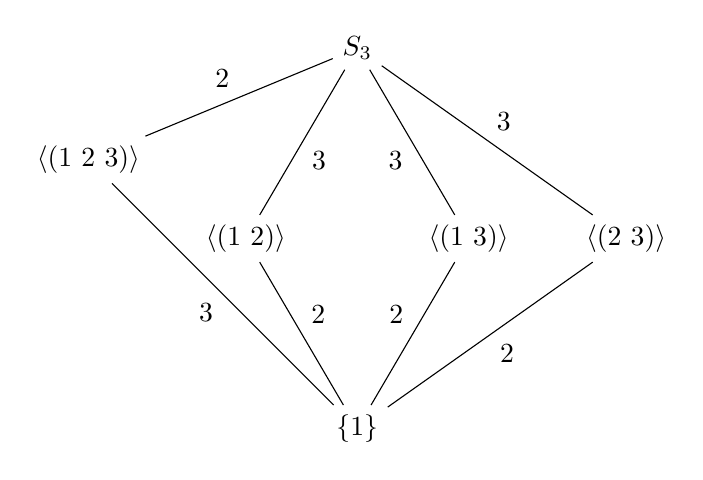
\begin{tikzpicture}[node distance=2cm]
                            \node (S3) {$S_3$};
                            \node (1) [below left of=S3, yshift=-1cm] {$\left\langle (1\ 2)\right\rangle$};
                            \node (2) [below right of=S3, yshift=-1cm] {$\left\langle (1\ 3)\right\rangle$};
                            \node (3) [left of=1, yshift=1cm] {$\left\langle (1\ 2\ 3)\right\rangle$};
                            \node (4) [right of=2] {$\left\langle (2\ 3)\right\rangle$};
                            \node (5) [below right of=1, yshift=-1cm] {$\{1\}$};
                            
                            \draw (S3) -- node[below right] {$3$} (1);
                            \draw (S3) -- node[below left] {$3$} (2);
                            \draw (S3) -- node[above left] {$2$} (3);
                            \draw (S3) -- node[above right] {$3$} (4);
                            \draw (1) -- node[above right] {$2$} (5);
                            \draw (2) -- node[above left] {$2$} (5);
                            \draw (3) -- node[below left] {$3$} (5);
                            \draw (4) -- node[below right] {$2$} (5);
                        \end{tikzpicture}
                        \caption{Diagrama de Hasse para los subgrupos de $S_3$.}
                    \end{figure}

                    Si observamos el retículo de subgrupos de $S_3$, observamos que hay 3 subgrupos distintos de orden 2, por lo que tendremos que $n_2 = 3$.

                \item Los $3-$subgrupos de Sylow será un subgrupo de orden 3 de $S_3$, que será el único que hay: $\langle (1\ 2\ 3) \rangle  = A_3 \lhd S_3$. 

                    Si queremos verlo por el Segundo Teorema de Sylow:
                    \begin{equation*}
                        \left.\begin{array}{r}
                            n_3 \mid 2 \\
                            n_3 \equiv 1 \mod 3
                    \end{array}\right\} \Longrightarrow n_3 = 1
                    \end{equation*}
                \end{itemize}
                \item En $A_4$, tenemos $|A_4| = 12 = 2^2 \cdot 3$. Tendremos:
                    \begin{itemize}
                        \item $2-$subgrupo de Sylow de orden 4. Busquemos por el Segundo Teorema de Sylow:
                            \begin{equation*}
                                \left.\begin{array}{r}
                                    n_2 \mid 3 \\
                                    n_2 \equiv 1 \mod 2
                            \end{array}\right\} \Longrightarrow n_2 \in \{1,3\}
                            \end{equation*}
                            Observando el retículo de $A_4$, concluimos que $n_2 = 1$, ya que el único subgrupo de orden 4 de $A_4$ es $V$, que es normal en $A_4$.
                        \item $3-$subgrupo de Sylow de orden 3:
                            \begin{equation*}
                                \left.\begin{array}{r}
                                    n_3 \mid 4 \\
                                    n_3 \equiv 1 \mod 3
                                \end{array}\right\} \Longrightarrow n_3 \in \{1,4\} 
                            \end{equation*}
                            Y observando el retículo de $A_4$, serán los 4 subgrupos de $A_4$ generados por los $3-$ciclos:
                            \begin{equation*}
                                \langle (1\ 2\ 3) \rangle  \qquad \langle (1\ 2\ 4) \rangle  \qquad \langle (1\ 3\ 4) \rangle  \qquad \langle (2\ 3\ 4) \rangle 
                            \end{equation*}
                    \end{itemize}
                \item En $S_4$, $|S_4| = 24 = 2^3 \cdot 3$:
                    \begin{itemize}
                        \item Para los $2-$subgrupos:
                            \begin{equation*}
                                \left.\begin{array}{r}
                                    n_2 \mid 3 \\
                                    n_2 \equiv 1 \mod 2
                                \end{array}\right\} \Longrightarrow n_2 \in \{1,3\}
                            \end{equation*}
                            Si suponemos que $n_2 = 1$, sea $Q<S_4$ un subgrupo con $|Q| = 8$, será el único $2-$subgrupo de Sylow. En dicho caso, todas las trasposiciones de $S_4$ deben estar contenidas en $Q$, ya que $\langle (x\ y) \rangle $ es un $2-$grupo (es un grupo de orden 2) y todo $2-$grupo está contenido en un $2-$grupo de Sylow (gracias al Segundo Teorema de Sylow), por lo que $Q$ contiene todas las trasposiciones. Sin embargo, como $S_4 = \langle \{(x\ y) \mid x,y \in \{1,2,3,4\}\} \rangle $, tendremos que $Q = S_4$, \underline{contradicción}.

                            Por tanto, tenemos $n_2 = 3$, tenemos tres $2-$subgrupos de Sylow: $Q_1$, $Q_2$ y $Q_3$. El grupo de Klein $V$ es un $2-$subgrupo, por lo que va a estar contenido en algún $Q_k$ (para $k \in \{1,2,3\}$). Supongamos que $V<Q_1$. Como todos ellos son conjugados, $\exists \alpha,\beta\in S_4$ de forma que:
                            \begin{align*}
                                Q_2 &= \alpha Q_1 \alpha^{-1} \\
                                Q_3 &= \beta Q_1 \beta^{-1} 
                            \end{align*}
                            Y si multiplicamos (como $V \lhd S_4$):
                            \begin{align*}
                                V = \alpha V \alpha^{-1} < \alpha Q_1 \alpha^{-1} = Q_2 \\
                                V = \beta V \beta^{-1} < \beta Q_1 \beta^{-1} = Q_3
                            \end{align*}
                            De donde deducimos que $V< Q_k$ para todo $k\in \{1,2,3\}$. Los $Q_k$ contendrán a $V$ y deben repartirse entre ellos a las trasposiciones. Realizando las cuentas pertinentes, podemos llegar a deducir que:
                            \begin{align*}
                                Q_1 &= V\langle (1\ 2) \rangle  \\
                                Q_2 &= V\langle (1\ 3) \rangle  \\
                                Q_3 &= V\langle (1\ 4) \rangle  
                            \end{align*}
                        \item Para los $3-$subgrupos de Sylow:
                            \begin{equation*}
                                \left.\begin{array}{r}
                                    n_3 \mid 8 \\
                                    n_3 \equiv 1 \mod 3
                                \end{array}\right\} \Longrightarrow n_3 \in \{1,4\}
                            \end{equation*}
                            Como sabemos de la existencia de varios elementos de orden 3, los $3-$subgrupos de Sylow de $S_4$ serán:
                            \begin{equation*}
                                \langle (1\ 2\ 3) \rangle , \langle (1\ 2\ 4) \rangle , \langle (1\ 3\ 4) \rangle , \langle (2\ 3\ 4) \rangle 
                            \end{equation*}
            \end{itemize}
    \end{itemize}
\end{ejemplo}

\begin{coro}
    Sea $P$ un $p-$subgrupo de Sylow de un grupo finito $G$. Entonces:
    \begin{equation*}
        P \text{\ es el único $p-$subgrupo de Sylow} \Longleftrightarrow P\lhd G
    \end{equation*}
    \begin{proof}
        Como en el Segundo Teorema de Sylow vimos que el conjugado de un $p-$subgrupo de Sylow es un $p-$subgrupo de Sylow y que todos los $p-$subgrupos de Sylow son conjugados entre sí, acabamos de justificar $(\ast)$ en::
        \begin{equation*}
            P \text{\ es el único $p-$subgrupo de Sylow de $G$} \stackrel{(\ast)}{\Longleftrightarrow} gPg^{-1} = P \quad \forall g\in G \Longleftrightarrow P\lhd G
        \end{equation*}
        La segunda equivalencia se tiene por una caracterización vista de los subgrupos normales.
    \end{proof}
\end{coro}

\begin{ejemplo}
    Todo grupo de orden 35 es resoluble.
    \begin{proof}
        Sea $G$ un grupo con $|G| = 35 = 5\cdot 7$, vemos que:
        \begin{equation*}
            \left.\begin{array}{r}
                n_7 \mid 5 \\
                n_7\equiv 1 \mod 5
            \end{array}\right\} \Longrightarrow n_7 = 1
        \end{equation*}
        En dicho caso, tenemos un único $7-$subgrupo de Sylow $H<G$, que tendrá orden 7 y por el Corolario anterior será normal en $G$. En dicho caso, sabemos que será isomorfo a $\mathbb{Z}_7$. Como los grupos abelianos son resolubles, tenemos que $H$ es resoluble. Si consideramos el cociente:
        \begin{equation*}
            |G/H| = \dfrac{|G|}{|H|} = \dfrac{5\cdot 7}{7} = 5
        \end{equation*}
        Por lo que $G/H\cong \mathbb{Z}_5$ y $G/H$ será resoluble por ser isomorfo a un grupo abeliano. Deducimos que $G$ es resoluble, por ser $H$ y $G/H$ resolubles.
    \end{proof}
    \noindent
    Esta estrategia que hemos seguido para demostrar que cualquier grupo de orden 35 es resoluble puede seguirse de forma análoga para demostrar que otros grupos de cierto orden son siempre resolubles.
\end{ejemplo}

\begin{teo}\label{teo:prod_grupos_sylow}
    Sea $G$ un grupo finito en el que todos sus subgrupos de Sylow son normales, entonces $G$ es el producto directo interno de sus subgrupos de Sylow:
    \begin{equation*}
        G = \prod_{H\in Syl(G)} H
    \end{equation*}
    \begin{proof}
        En la caracterización de producto directo interno para una cantidad finita de subgrupos (Teorema~\ref{teo:prod_dir_int_fam}), vimos que $G$ era producto directo interno de todos ellos (los llamaremos $H_i$ con $i \in \{1,\ldots,n\}$) si y solo si:
        \begin{itemize}
            \item $H_i \lhd G$ para todo $i \in \{1,\ldots,n\}$.
            \item $H_1H_2\ldots H_n = G$.
            \item $(H_1\ldots H_{i-1}) \cap H_i = \{1\}$, para todo $i \in \{2,\ldots,k\}$
        \end{itemize}
        Basta pues, demostrar estos 3 puntos. Supuesto que $|G| = p_1^{n_1} \ldots p_k^{n_k}$, llamamos $P_i$ al único $p_i-$subgrupo de Sylow, para todo $i \in \{1,\ldots,k\}$.

        \begin{itemize}
            \item Por hipótesis, tendremos que $P_i \lhd G$ para todo $i \in \{1,\ldots,k\}$.
            \item También:
                \begin{equation*}
                    |P_1P_2 \ldots P_K| = |P_1||P_2|\ldots |P_k| = |G|
                \end{equation*}
                Y como tenemos siempre que $P_1P_2\ldots P_k < G$, deducimos que $P_1P_2\ldots P_k = G$.
            \item Fijado $i \in \{2,\ldots,k\}$, veamos que $(P_1 \ldots P_{i-1}) \cap P_i = \{1\}$. Para ello, sea $x\in (P_1 \ldots P_{i-1}) \cap P_i$, tenemos:
                \begin{equation*}
                    \left.\begin{array}{l}
                        O(x) \mid |P_1\ldots P_{i-1}| = p_1^{n_1} \ldots p_{i-1}^{n_{i-1}} \\
                        O(x) \mid |P_i| = p_i^{n_i}
                    \end{array}\right\} \Longrightarrow O(x) = 1 \Longrightarrow x = 1
                \end{equation*}\qedhere
        \end{itemize}
    \end{proof}
\end{teo}

\begin{observacion}
    Notemos que cualquier grupo abeliano finito es producto directo interno de sus subgrupos de Sylow, ya que el Primer Teorema de Sylow nos garantiza su existencia y por ser el grupo abeliano siempre tendremos que dichos subgrupos son normales.
\end{observacion}
